% !TEX root = ../elsarticle-template.texmain.tex
%-------------------
\section{Case study: Finite State Machines}
\label{sec:validation}

 To evaluate of our approach, we use as case study the set of DSLs for state machines. Note that a simplified version have been used as running example along this paper (see Section \ref{sec:thedevelopmentscenario}). This case study is inspired from the analysis of variability on languages for finite state machines provided by Crane et al. \cite{Crane:2007}, and it is composed of three different DSLs: UML state diagrams, Rhapsody, and Harel's state charts. As aforementioned, these DSLs have some commonalities since they are intended to express the same formalism. According to the development scenario we address in this paper, these commonalities will be materialized as clones in the DSL specifications. In this section, we summarize both commonalities and differences existing in the case study. Then, we apply our approach and we present the obtained results. To explain this case stude we followed a mehod inspired by Runeson et al\cite{runeson-book}.

\subsection{Background to the research project}
This research is the result of a bilateral collaboration (2011 - 2015) between the DiverSE team at INRIA and the MDE lab at Thales Research & Technology (TRT) in the framework of the VaryMDE project. This partnership explores variability management issues at both the modeling level and the metamodeling level (i.e., design and implementation of software languages).

As a matter of fact, while DSLs have been found useful for structuring development processes and providing abstractions to stakeholders, their ultimate value has been severely limited by the cost of the associated tooling (i.e., editors, parsers, etc...). The construction of that tooling is a challenging and time-consuming task that requires specialized knowledge. A language designers must own not only quite solid modeling skills but also the technical expertise for conducting the definition of specific artifacts such as grammars, metamodels, compilers, and interpreters. The situation becomes even more difficult in the context of multi-domain companies (such as Thales) where there are several domains that co-exist and overlap through different business units. In that case, diverse, and possibly conflicting, requirements often appear on the same DSL specially when it is required by two or more business units. According to its modeling needs, each business unit imposes specific constraints and demands particular capabilities. Language designers must face these situation by adapting the DSL and releasing different variants when needed.

The typical development process to address the aforementioned situation is quite similar to the one followed in the
general case of software development: at the beginning, there is a first DSL from which new development branches are forked and where the DSL is adapted to the new requirements. After some repetitions, language designers have a set of DSLs (a.k.a family of DSLs) that share some commonalities (materialized as replication of code) and that offer different capabilities that have been adapted for the application context. As one may expect, this approach introduces several problems. For example, because of code replication, all the effort invested in maintenance and bug fixing should be replicated as well.

In this context, it is desirable to have an approach that facilitates the engineering of families of DSLs. Such approach should be intended to exploit reuse as an alternative to code replication and to manage the variability among the different DSLs that compose the family. In addition, it is worth noting that an approach for dealing with families of DSLs has to take into account that the differences among members of a family of DSLs can be found in at any of the implementation concerns.


\subsection{Case Study Design and planning}
\subsubsection{Rationale}
The retionale behind this study is to contribute to the state of the art of DSL development. We want to discover if in an industrial case such as the one involving the VaryMDE project we can reverse engeniering language madules and then, improve the develoment process for future DSLs.

\subsubsection{Objective}
The main objective of this case study is to analyse the amount of reuse automatically retrieved from the software artifacts.
\subsubsection{Units of Analyses}
Two main units of analysis has been considered. First, the commonalities, this is the common parts to all the existing state machines formalisms. Second, the variabilities


\paragraph{Description of the Commonalities}

Generally speaking, state machines are graphs where nodes represent states and arcs represent transitions between the states \cite{Harel:1987}. The execution of a state machine is performed in a sequence of \textit{steps} each of which receives a set of events that the state machine should react to. The reaction of a machine to set of events can be understood as a passage from an initial configuration (t$_i$) to a final configuration (t$_{f}$). A configuration is the set of active states in the machine.

The relationship between the state machine and the arriving events is materialized at the level of the transitions. Each transition is associated to one or more events (also called triggers). When an event arrives, the state machine fires the transitions outgoing from the states in the current configuration whose trigger matches with the event. As a result, the source state of each fired transition is deactivated whereas the corresponding target state is activated. Optionally, guards might be defined on the transitions. A transition is fired if and only if the evaluation of the guard returns true at the moment of the trigger arrival.

The initial configuration of the state machine is given by a set of initial pseudostates.  Transitions outgoing from initial pseudosates are fired automatically when the state machine is initialized. In turn, the execution of a state machine continues until the current configuration is composed only by final states (an special type of states without outgoing transitions).

All of the DSLs included in this case study support the notion of region. A state machine might be divided in several regions that are executed concurrently. Each region might have its own initial and final (pseudo)states. In addition, the DSLs also support the definition of different types of actions. States can define entry/do/exit actions, and transitions can have effect actions.

\paragraph{Description of the Variability}

\vspace{2mm}
\textit{\textbf{Abstract syntax variability.}} Differences at the level of the abstract syntax between the DSLs under study correspond to the diversity of constructs each of those DSLs provide. In particular, there are differences in the support for transition's triggers and pseudostates.

In the case of transitions' triggers, whereas Rhapsody only supports atomic triggers, both Harel's statecharts and UML provide support for composite triggers. In Harel's statecharts triggers can be composed by using \texttt{AND}, \texttt{OR}, and \texttt{NOT} operators. In turn, in UML triggers can be composed by using the \texttt{AND} operator.

In the case of pseudostates, whereas all the DSLs support \texttt{Fork}, \texttt{Join}, \texttt{ShallowHistory}, and \texttt{Junction}, there are two psueudostates i.e., \texttt{DeepHistory} and \texttt{Choice} that are only supported by UML. The \texttt{Conditional} pseudostate is only provided by Harel's state charts. Table \ref{fig:oracle} shows the language constructs provided by each DSL.

\begin{table*}[t]
\centering
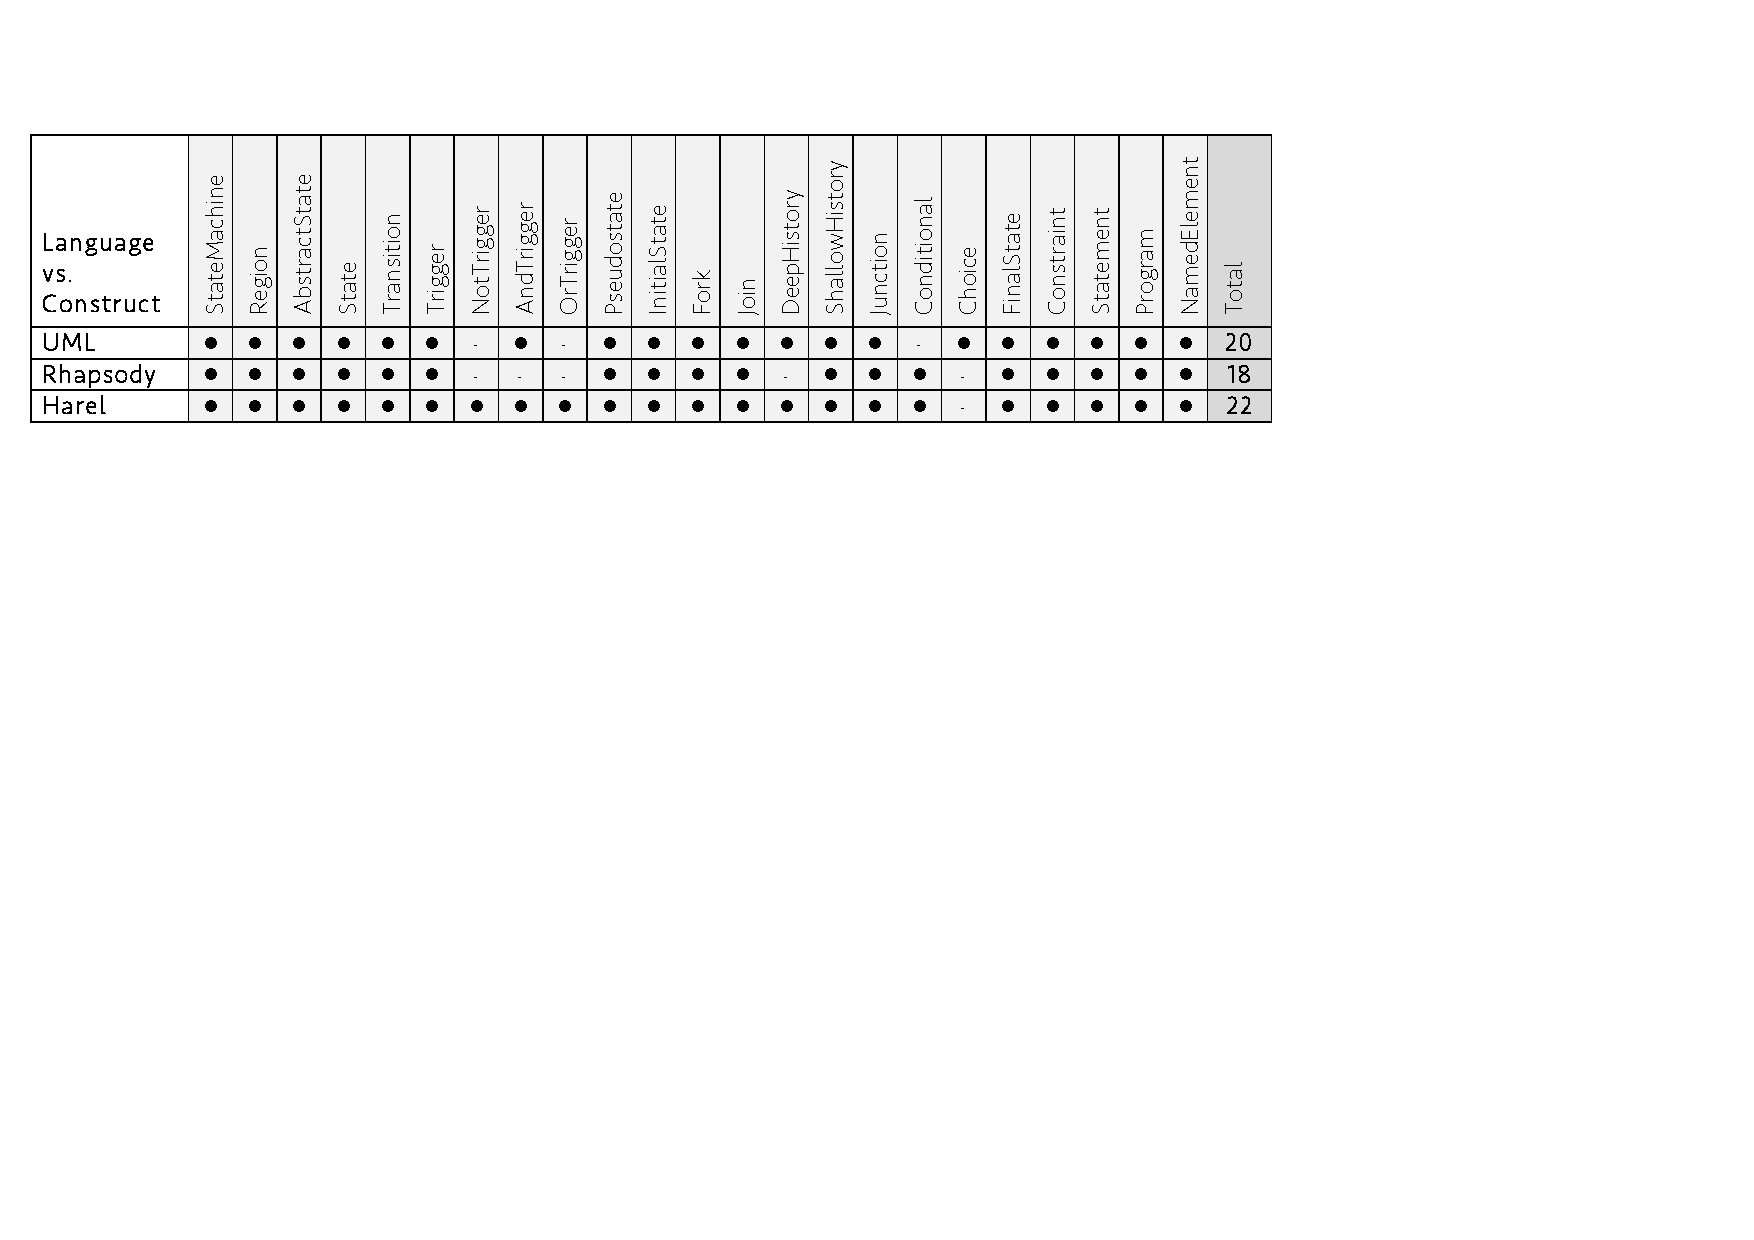
\includegraphics[width=1\linewidth]{images/tab-oracle-statemachines}
\caption{Diversity of constructs provided by the DSLs for state machines}
\label{fig:oracle}
\end{table*}

\vspace{2mm}
\textit{\textbf{Semantic variability.}} Semantic differences between the DSLs under study can be summarized in three issues:

\vspace{2mm}
\textit{(1) Events dispatching policy:} The first semantic difference in the operational semantics of state machines refers to the way in which events are consumed by the state machine. In a first interpretation, simultaneous events are supported i.e., the state machine can process more than one event in a single step. In a second interpretation, the state machine follows the principle of run to completion i.e., the state machine is able only of supporting one event by step so several events require several steps.

The semantics of UML and Rhapsody fit the run to completion policy for events dispatching whereas Harel's statecharts support simultaneous events.

\vspace{2mm}
\textit{(2) Execution order of transitions' effects:} It is possible to define actions on the transitions that will affect the execution environment where transitions are fired. These actions are usually known as transitions' effects. All the DSLs for state machines in our family support the expression of such effects. However, there are certain differences regarding their execution.

The first way of executing the effects of a transition is by respecting the order in which they are defined. This is due to the fact that transitions effects are usually defined by means of imperative action script languages where the order of the instructions is intrinsic. The second interpretation to the execution of transitions' effect is to execute them in parallel. In other words, the effects are defined as a set of instructions that will be executed at the same time so no assumptions should be made with respect to the execution order.

UML and Rhapsody execute the transition effects in parallel. Harel's statecharts execute transition effects simultaneously.

\vspace{2mm}
\textit{(3) Priorities in the transitions:} Because several transitions can be associated to the same event, there are cases in which more than one transitions are intended to be fired in the same step. In general, all the DSLs for state machines agree in the fact that all the activated transitions should be fired. However, this is not always possible because conflicts might appear. Consider the state machine presented in Fig \ref{fig:conflicting-priorities}. The transitions $T_D$ and $T_E$ are conflictive because they are activated by the same event i.e., $e_2$, they exit the same state, and they go to different target states. Then, the final configuration of the state machine will be different according to the selected transition.

\begin{figure}[h!]
  \centering
  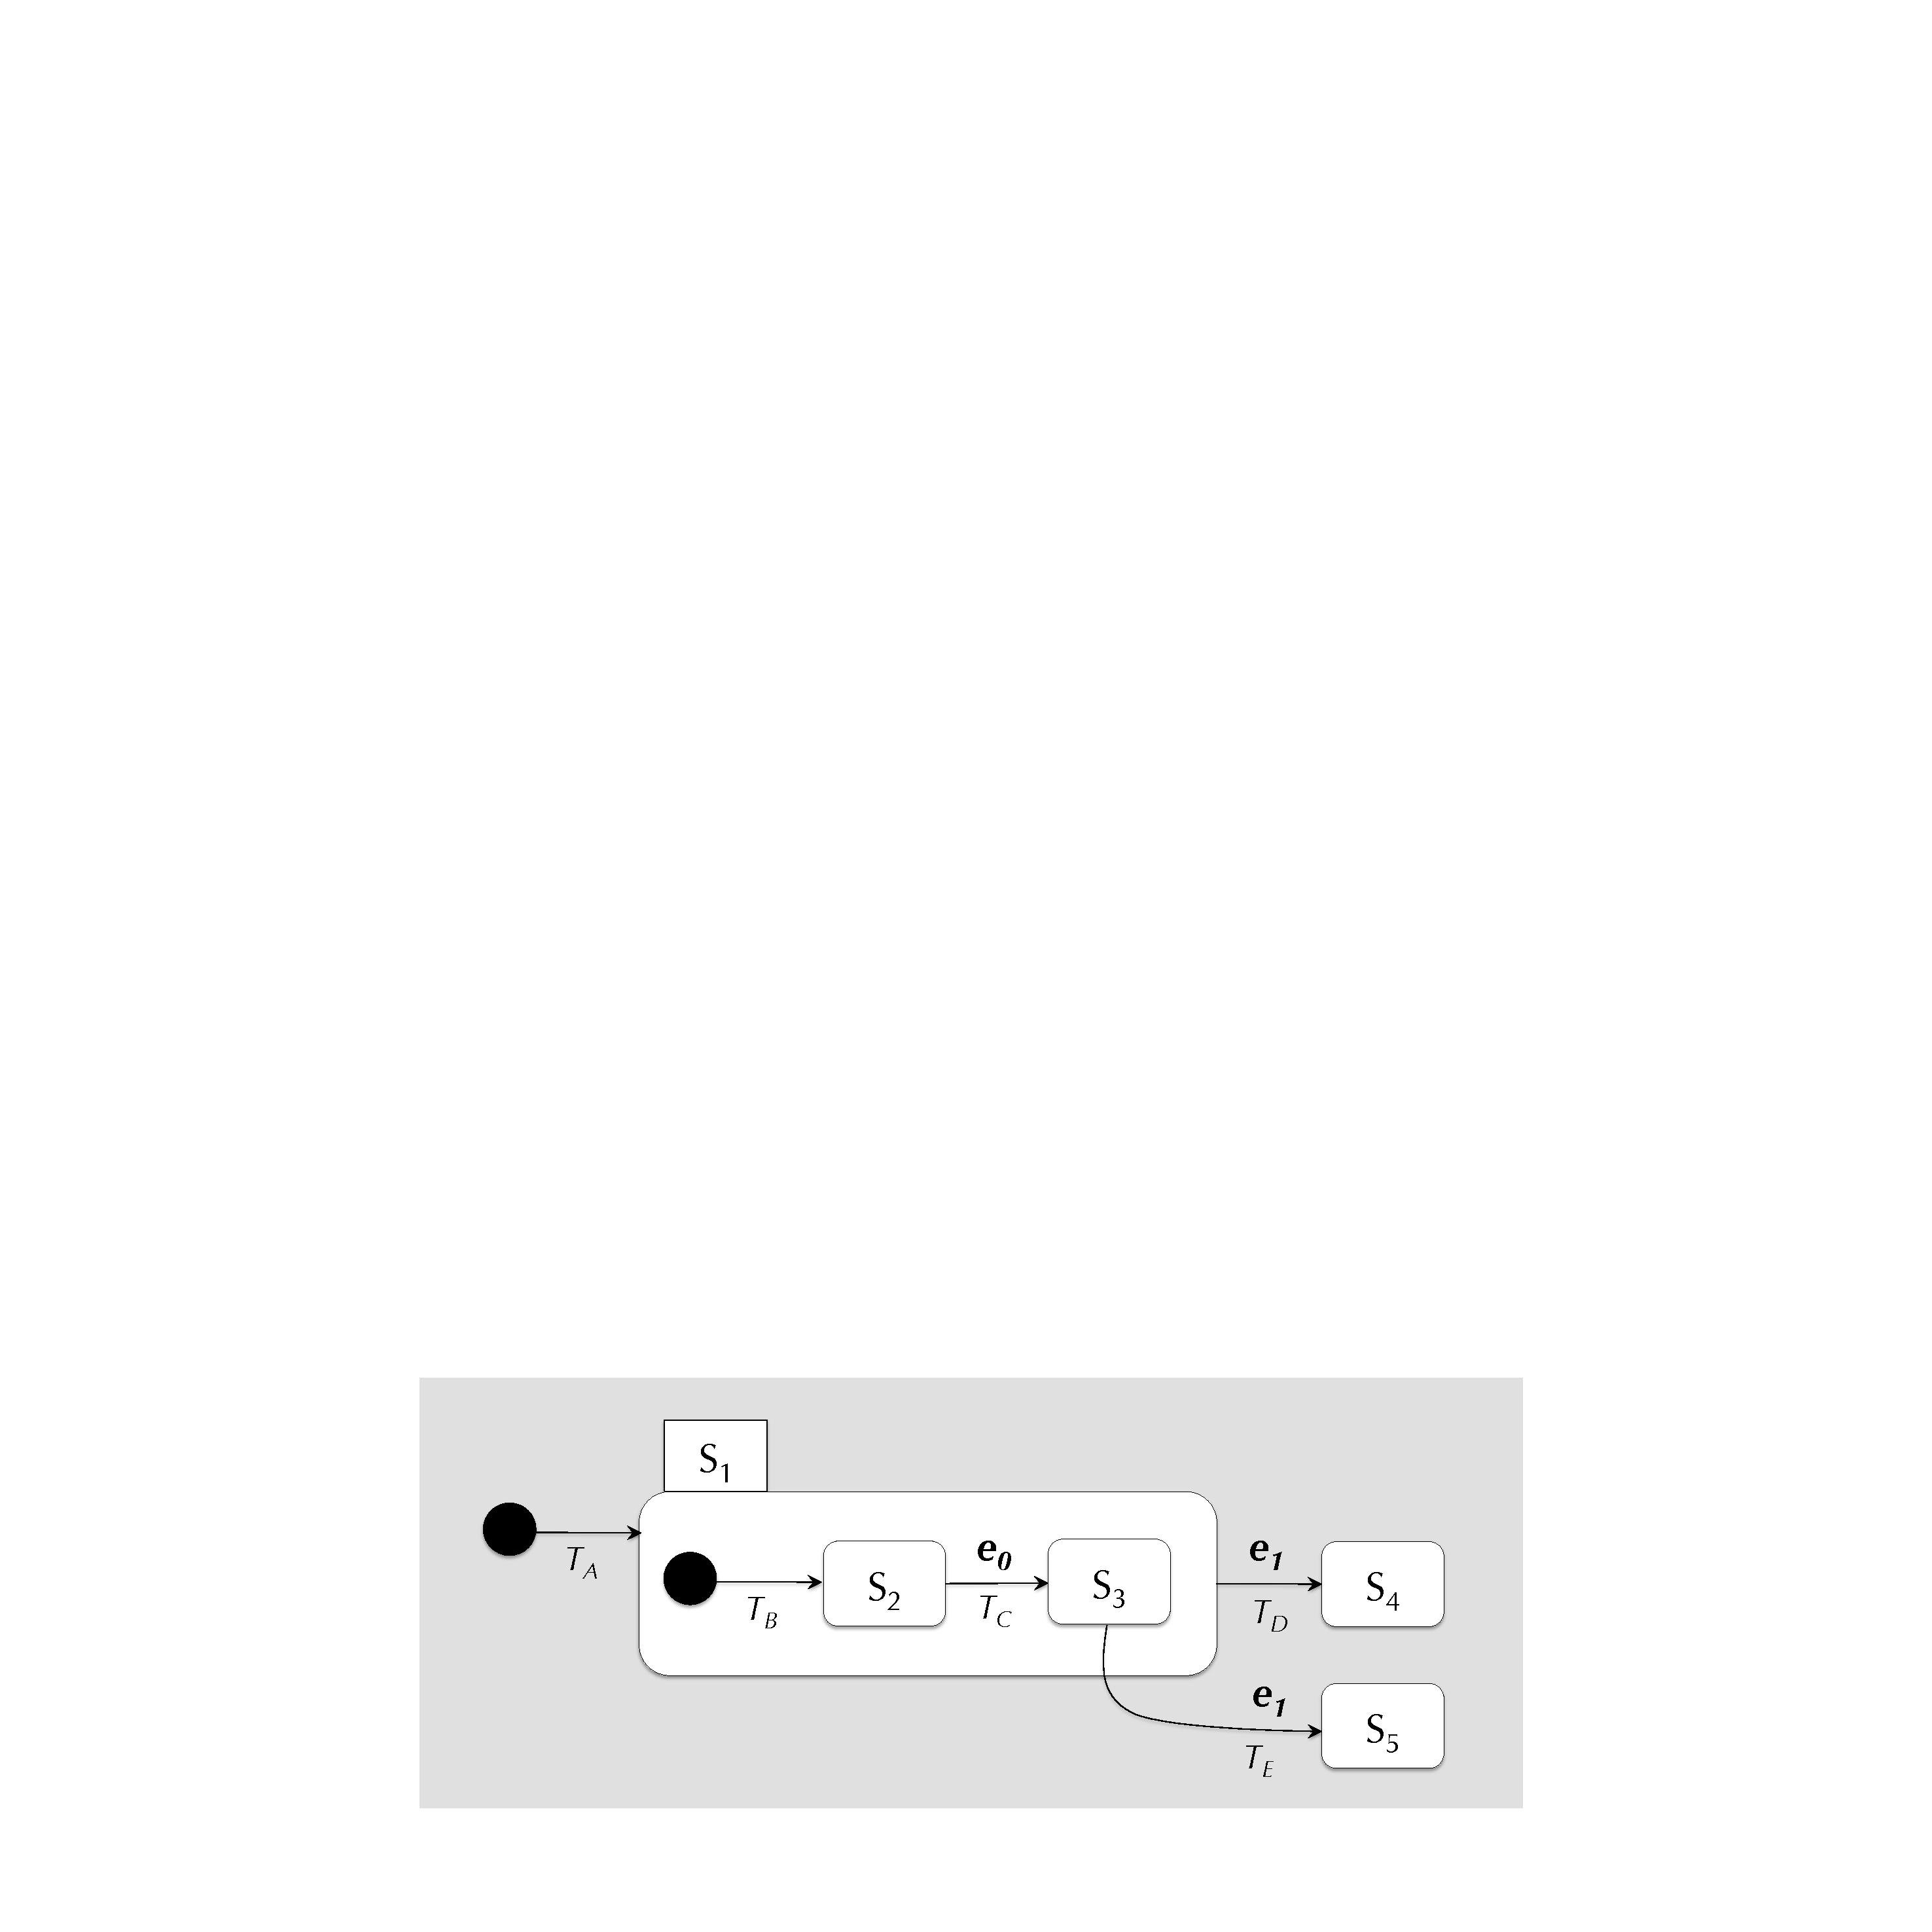
\includegraphics[width=1\linewidth]{images/conflicting-priorities.pdf}
  \caption{Example of a state machine with conflicting priorities}
  \label{fig:conflicting-priorities}
\end{figure}

To tackle this situation, it is necessary to establish policies that permit to solve such conflicts. Specifically, we need to define a mechanism for prioritizing conflicting transitions so the interpreter is able to easily select a transition from a group of conflicting transitions. One of the best known semantic differences among DSLs for state machines is related with these policies. In particular, there are two different mechanisms for solving this kind of conflicts. A first mechanism for solving conflicting transition is to select the transition with the lower scope. That is, the deeper transition w.r.t. the hierarchy of the state machine.

In the example presented in Fig \ref{fig:conflicting-priorities} the dispatched transition according to this policy would be the transition $T_E$ so the state machine would move to the state $S_5$. The second mechanism for solving conflicts in the transition is to select the transition with the higher scope. That is, the higher transition w.r.t. the hierarchy of the state machine. In the example presented in Fig \ref{fig:conflicting-priorities} the dispatched transition according to this policy is the transition $T_D$ so the state machine will move to the state $S_4$.

The semantics of UML and Rhapsody fits on the first interpretation i.e., deepest transition priority whereas the semantics of Harel's statecharts fits on the second interpretation i.e., highest transitions priority.

%are reified by the fact that not all the DSLs have the same behavior at execution time. For example, whereas Harel's statecharts attend simultaneous events in parallel, both UML and Rhapsody follow the run to completion principle. So, simultaneous events are attended sequentially \cite{Crane:2007}. Consequently, not all the domain-specific actions are the same. In particular, the domain-specific actions \texttt{eval()} and \texttt{step()} in the \texttt{StateMachine} metaclass are different in each DSL.
\subsubsection{Case Study protocol}

\subsection{Data collection}



\subsection{Results}

The starting point of the applicability of our approach in the case study is a set of DSLs implementing each of the specifications explained above. Hence, at the beginning we have three different DSLs for state machines that can be accessed in a \texttt{GitHub} repository\footnote{GitHub repository for the case study: \url{https://github.com/damende/puzzle/tree/master/examples/state-machines}}. Using these specifications as input, we proceed to apply our approach.

The results are summarized in Fig. \ref{fig:results-casestudy}. At the left of the figure we present the set of language modules we obtained as well as the language interfaces existing among them. Those modules group the language constructs according to the heuristic introduced in Section \ref{sec:reverseengineeringmodules} on breaking down intersections. At the right of the figure we show the corresponding variability models. Each feature of the feature models is associated to a given language module. In turn, the semantic variability points in the orthogonal model are associated to clusters of domain specific actions.

%Note that we marked different configurations in the figure to identify each of the corresponding DSLs. In addition, we calculated the number of possible configurations. We obtained that with this variability model, we can obtain XXX DSLs for state machines.

\begin{figure*}
\centering
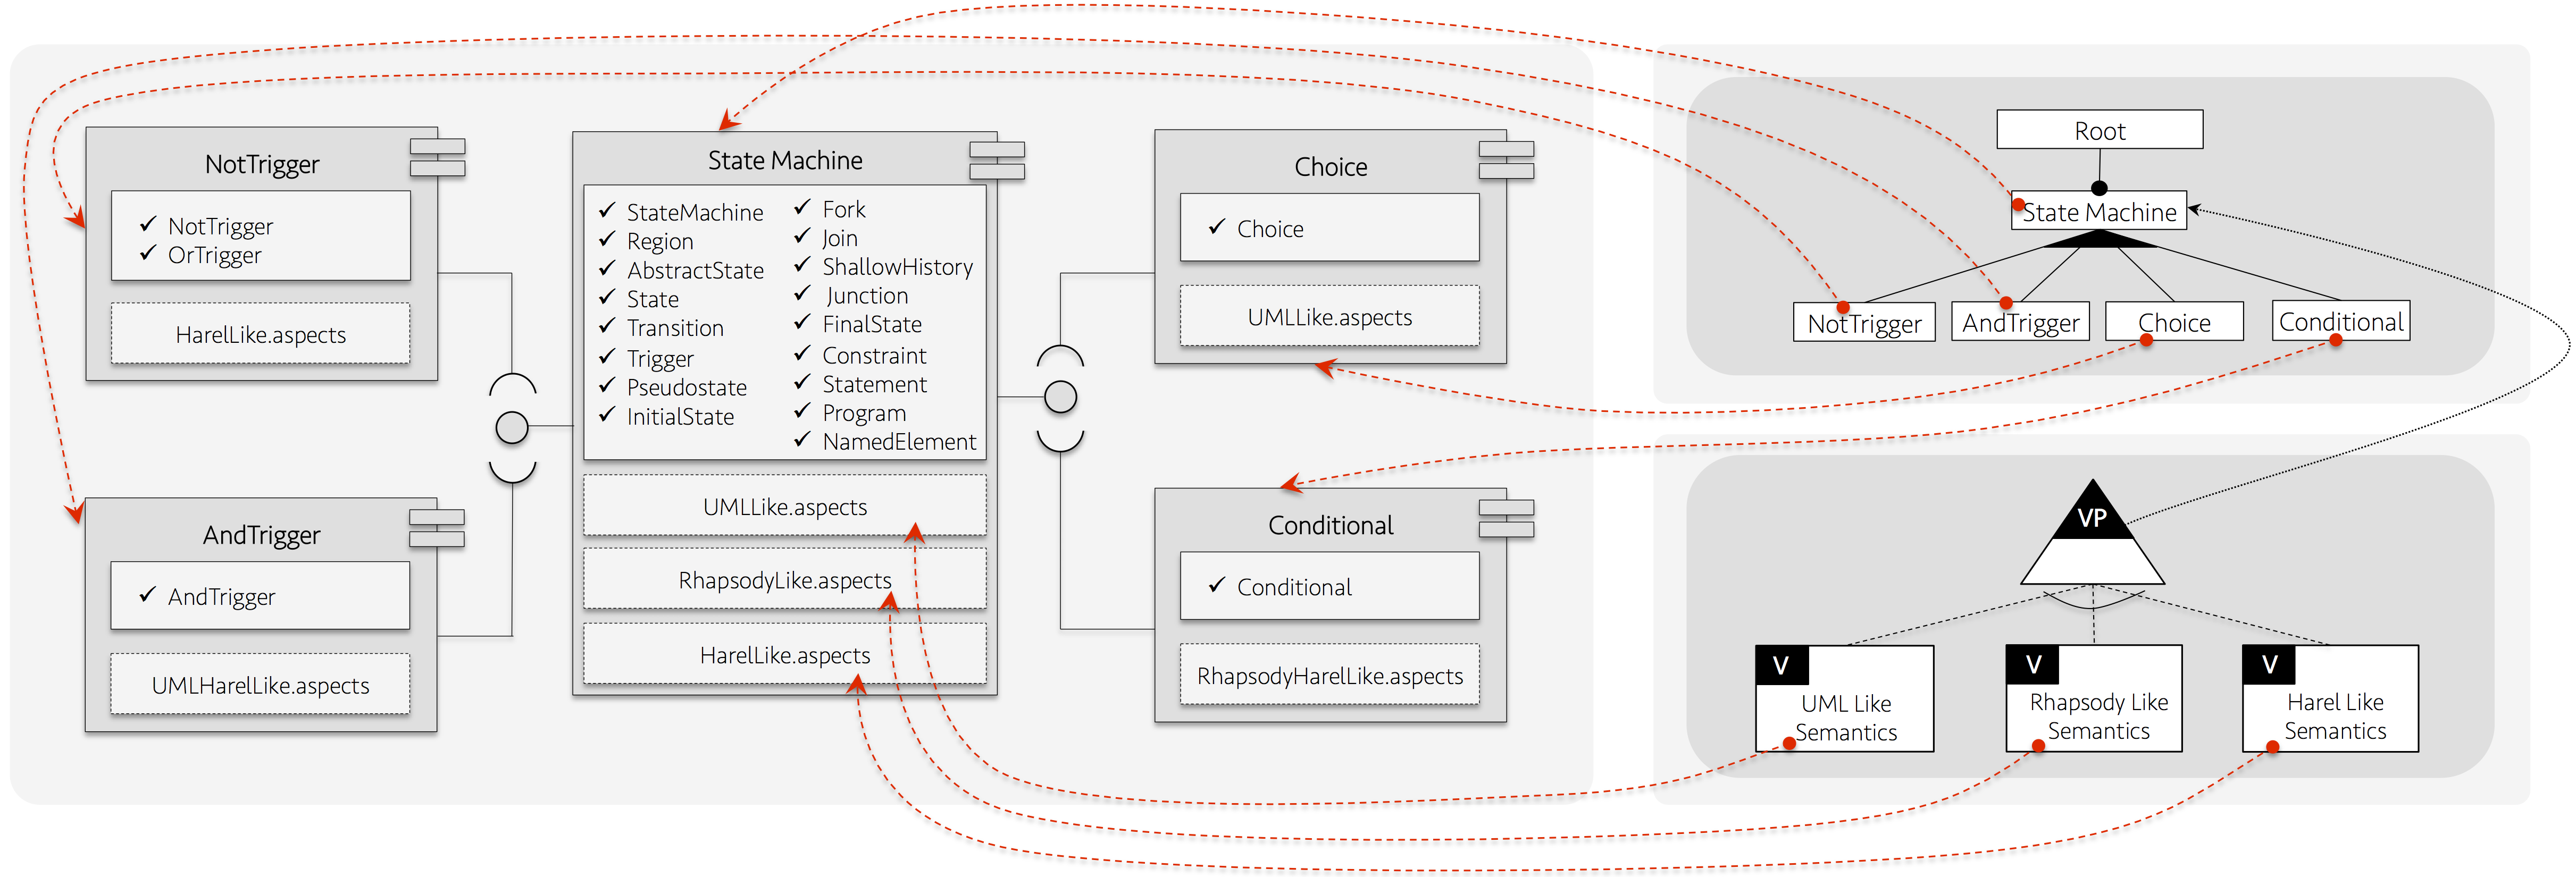
\includegraphics[width=1\linewidth]{images/results-casestudy.png}
\caption{Language product line produced for the case study of the finite state machines. }
\label{fig:results-casestudy}
\end{figure*}

\vspace{2mm}
\textbf{\textit{Analysis of the results.}} Let us now discuss the results of the case study. As expected, we obtained a language product product line from a set of DSL variants for finite state machines. But... Does this product line identify all the variation points and commonalities existing in the DSL variants? Are those variation points properly specified in the language modular design and variability models? Since we know these variation points and commonalities, we can check whether they are appear in the produced language product line. The results of this verification are presented in Table \ref{fig:validation-results}.

The results are promising in the case of abstract syntax variability. According to the Table \ref{fig:oracle}, the DSL variants share 17 constructs in common. Those constructs are properly factorized in a language module that we named StateMachine. This module is correctly identified during the recovering of the language modular design, and it is properly specified as a language module in terms of a metamodel enhance with domain specific actions and offering a provided interface. Besides, the particularities of the DSL variants are also well factorized. There is a module that contains the constructs NotTrigger and OrTrigger that belong only to the variant complying the Harel' statecharts specification. Besides, there are three additional modules that contain the constructs AndTrigger, Choice, and Conditional respectively. Using this modular design, we can re-compose any of the three initial DSL variants.

The situation is different for the case of semantic variability. Although our reverse-engineering strategy is able to identify that the domain specific actions are different in the three DSL variants, the level of granularity at which those variation points are detected is coarser than one might expect. At the beginning of this section, we described three semantic variation points and their possible interpretations i.e., events dispatching policy, execution order of transitions' effects, and priorities of conflicting transitions. Using the proposed technique, we can identify just one semantic variation point indicating that the language module called StateMachines contains three different clusters of domain specific actions, which is reflected in the orthogonal variability model.

This threat to validity of our technique can be explained by the fact that the analysis of commonalities and variability is conducted by means of static analysis. We can analyze the structure of the metamodels and the domain specific actions, but not their behavior at runtime. Hence, we cannot see how these differences impact the execution of the models. For example, we cannot infer that the differences among the domain specific actions in the StateMachine module impact the way in which conflicting priorities are managed. A next step in this research could be to use also dynamic analysis in the domain specific actions to better specify semantic variation points.

\begin{table}
\centering
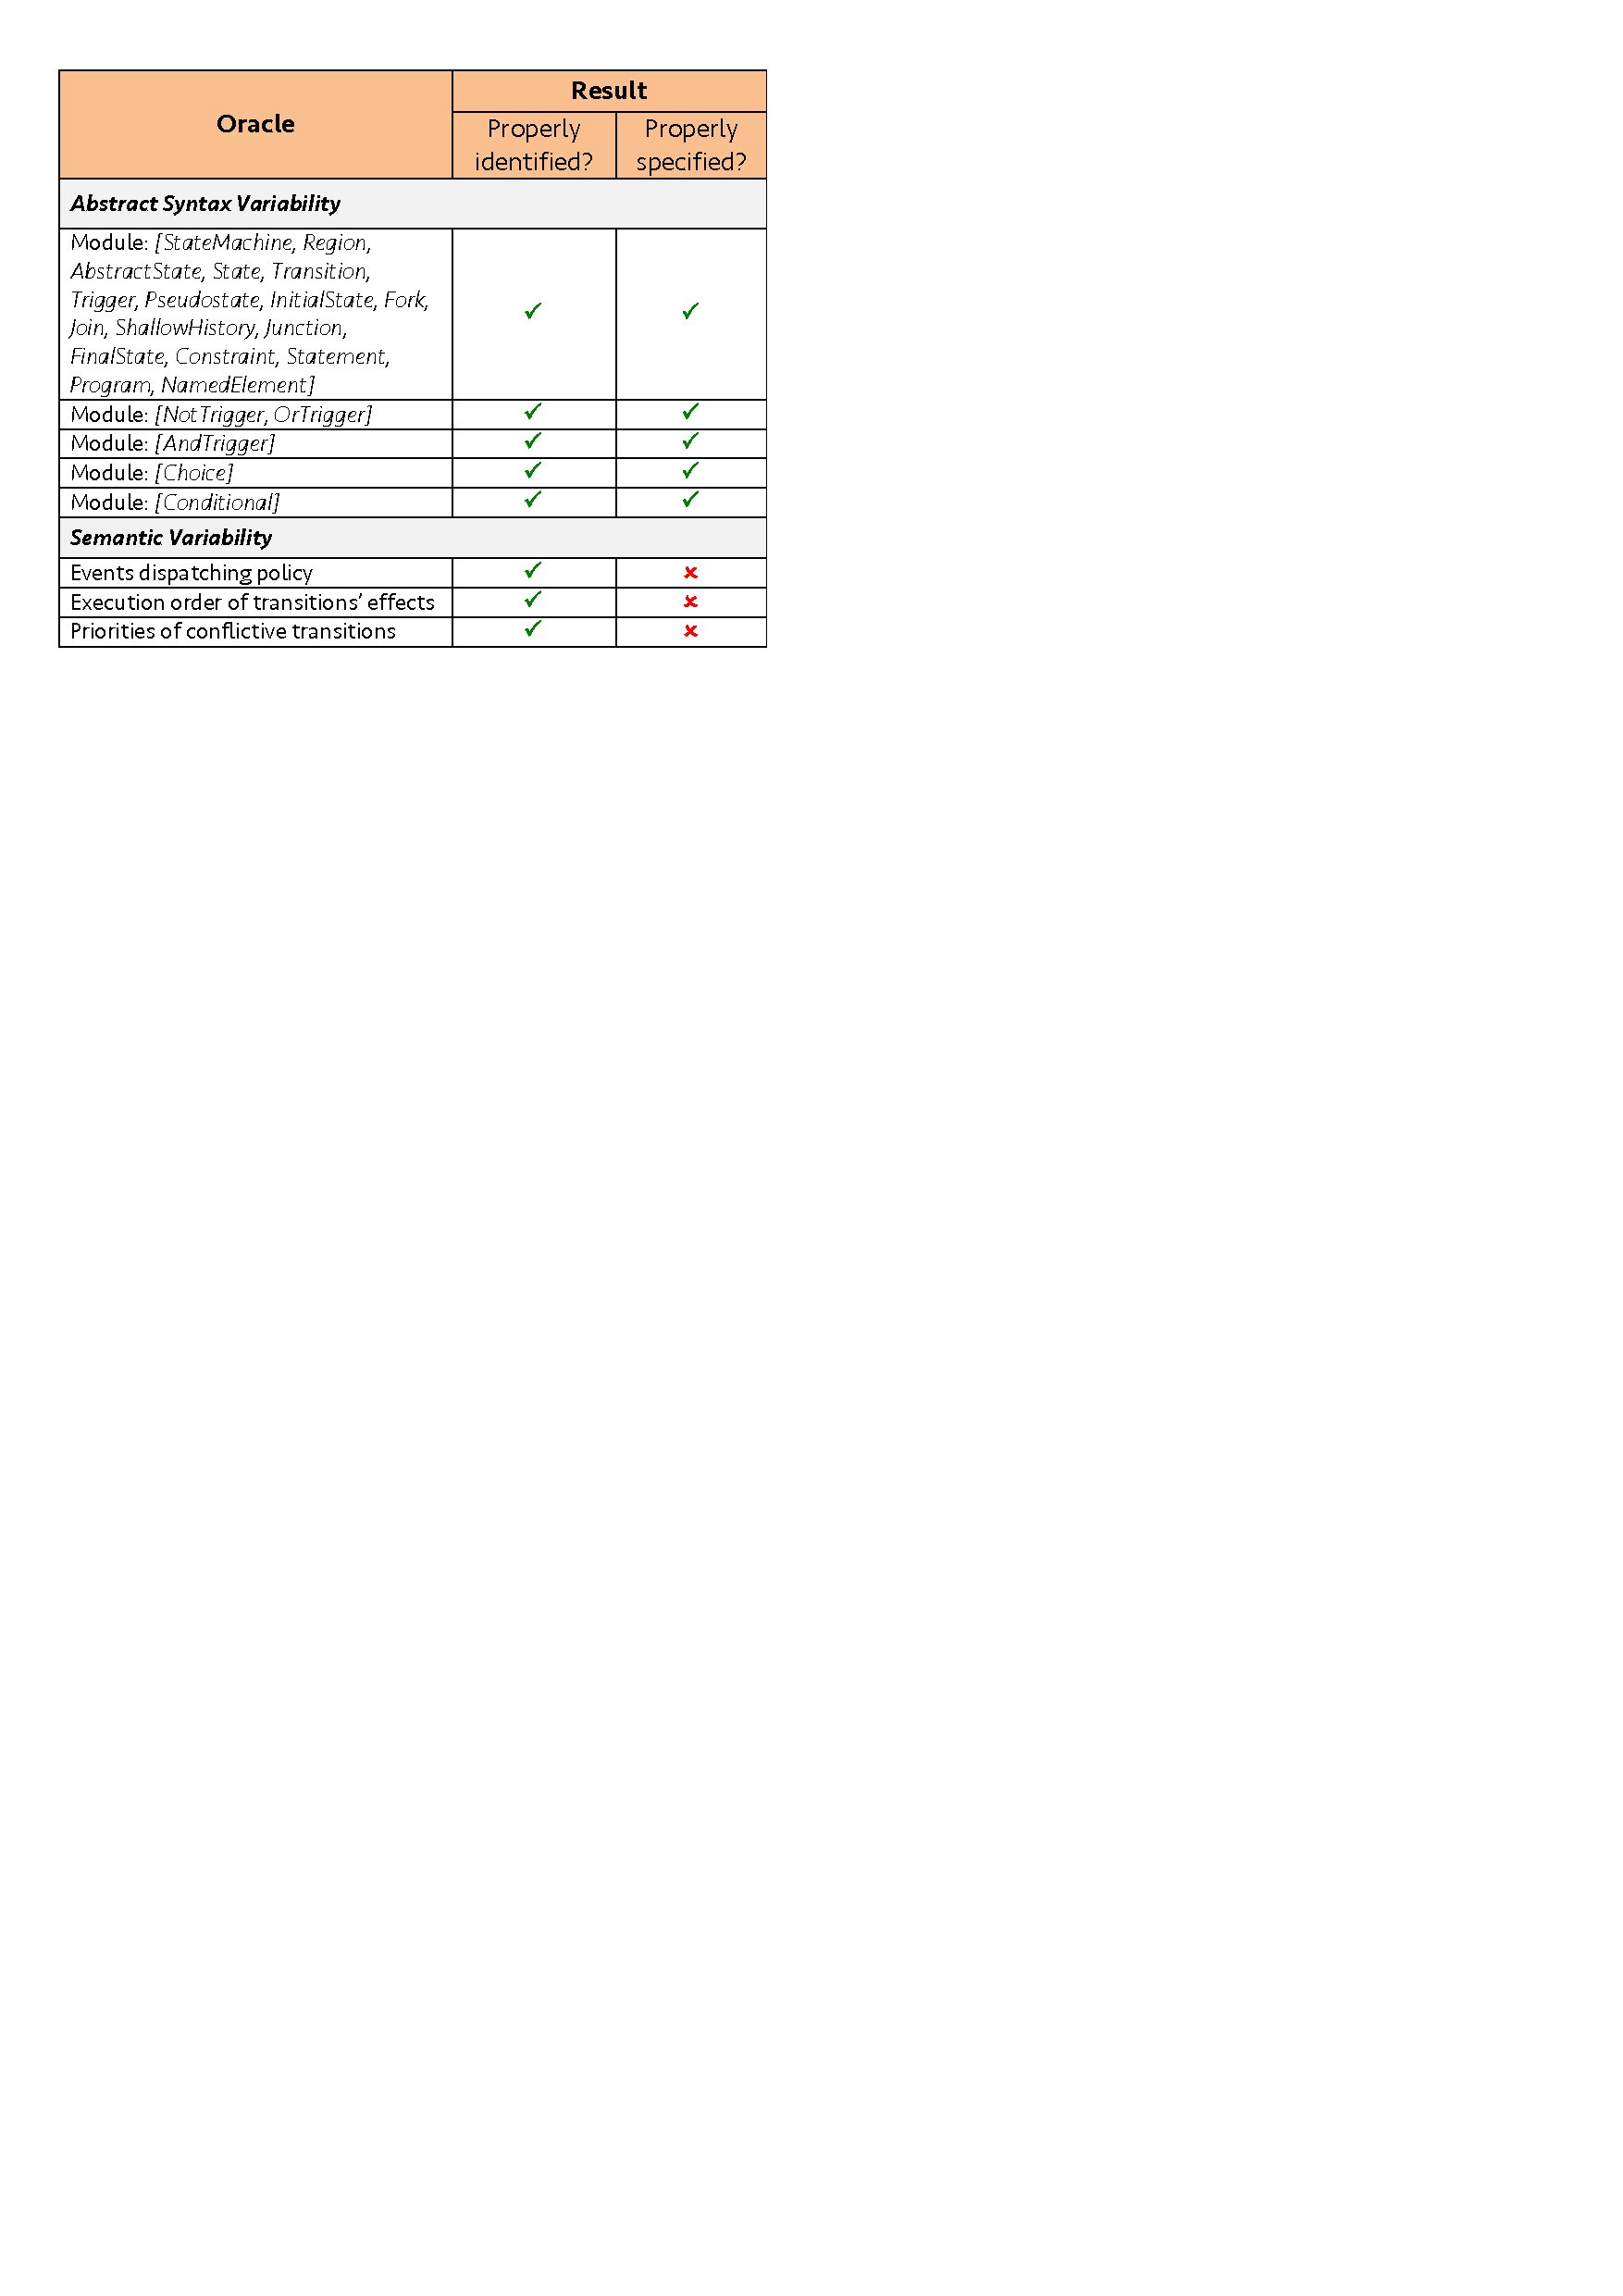
\includegraphics[width=1\linewidth]{images/validation-results}
\caption{Analysis of the results of the case study}
\label{fig:validation-results}
\end{table}
